\section{Ontologias Probabilísticas}
\label{sec:prob_ontology}

Para lidar com a incerteza da web atual foi desenvolvido o conceito de Ontologias Probabilísticas que além de ter as mesmas componentes que as mencionadas na seção~\ref{sec:ontology}, são adicionadas algumas características:

\begin{itemize}
	\item Regularidades estatísticas particulares do domínio
	\item Conhecimento ambíguo, incompleto e não confiável relacionado às entidades
	\item Incerteza sobre todas as formas anteriores de conhecimento (e.g. propriedades, classes, etc.)
\end{itemize}

Durante alguns anos, foram consideradas algumas representações existentes na época para tentar representar ontologias probabilísticas como será visto nas seguintes subseções, mas cada uma delas tinha problemas para lidar tanto com lógica como incerteza~\cite{Costa10}.

\subsection{Redes Bayesianas}
\label{subsec:bn}

Uma rede Bayesiana é um modelo gráfico sobre variáveis (aleatórias) conformada por um grafo direcionado acíclico e uma distribuição de probabilidades conjunta sobre todas as variáveis, estabelecendo independenças condicionais entre elas. Apesar de usar probabilidades e poder lidar com incerteza, sua estrutura é limitada por uma representação atributo-valor. Isto não permite que sejam usadas sentenças gerais da lógica (e.g. $paiDe( X )$).

\subsection{Modelos Ocultos de Markov}
\label{subsec:hmm}

Um modelo oculto de Markov é um caso particular de redes Bayesianas dinâmicas. Este tipo de redes adicionam uma variável de tempo a cada um dos valores nela. Apesar que Isto permite que podam ser usadas sentenças recursivas como na lógica, como no caso anterior, esta estrutura também está limitada pela representação atributo-valor.

\subsection{Modelos relacionados probabilísticos}
\label{subsec:prm}

Estes modelos extendem as redes Bayesianas para trabalhar com tipos de entidades, que é um dos componentes das ontologias e que as estruturas anteriores não conseguiam fazer diretamente. Ainda assim, o problema é que não conseguem ser usadas para representar sentenças com quantificadores (e.g. $\forall paiDe( X , Y ) \rightarrow filhoDe( Y , X )$).

\subsection{Multi-Entity Bayesian Networks}
\label{subsec:mebn}

Finalmente, no ano 2008, Laskey conseguiu desenvolver a primeira representação que combina lógica com incerteza de forma satisfatória. Aquela representação está baseada em um tipo de rede Bayesiana chamado Multi-Entity Bayesian Network (MEBN) onde cada sentença em lógica de primeira ordem pode ser representada como um fragmento ou MFrag como se mostra na Figura~\ref{fig:sentences}. Portanto, permite variáveis não instanciadas, quantificadores e recursão. Cada um desses fragmentos tem distribuições de probabilidades locais e o conjunto de MFrags construi toda a base de conhecimento chamada MTheory~\cite{Laskey08}. Na seguinte seção será usada esta estrutura para desenvolver a linguagem padrão PR-OWL para representar ontologias probabilísticas.

\begin{figure}
	\centering
	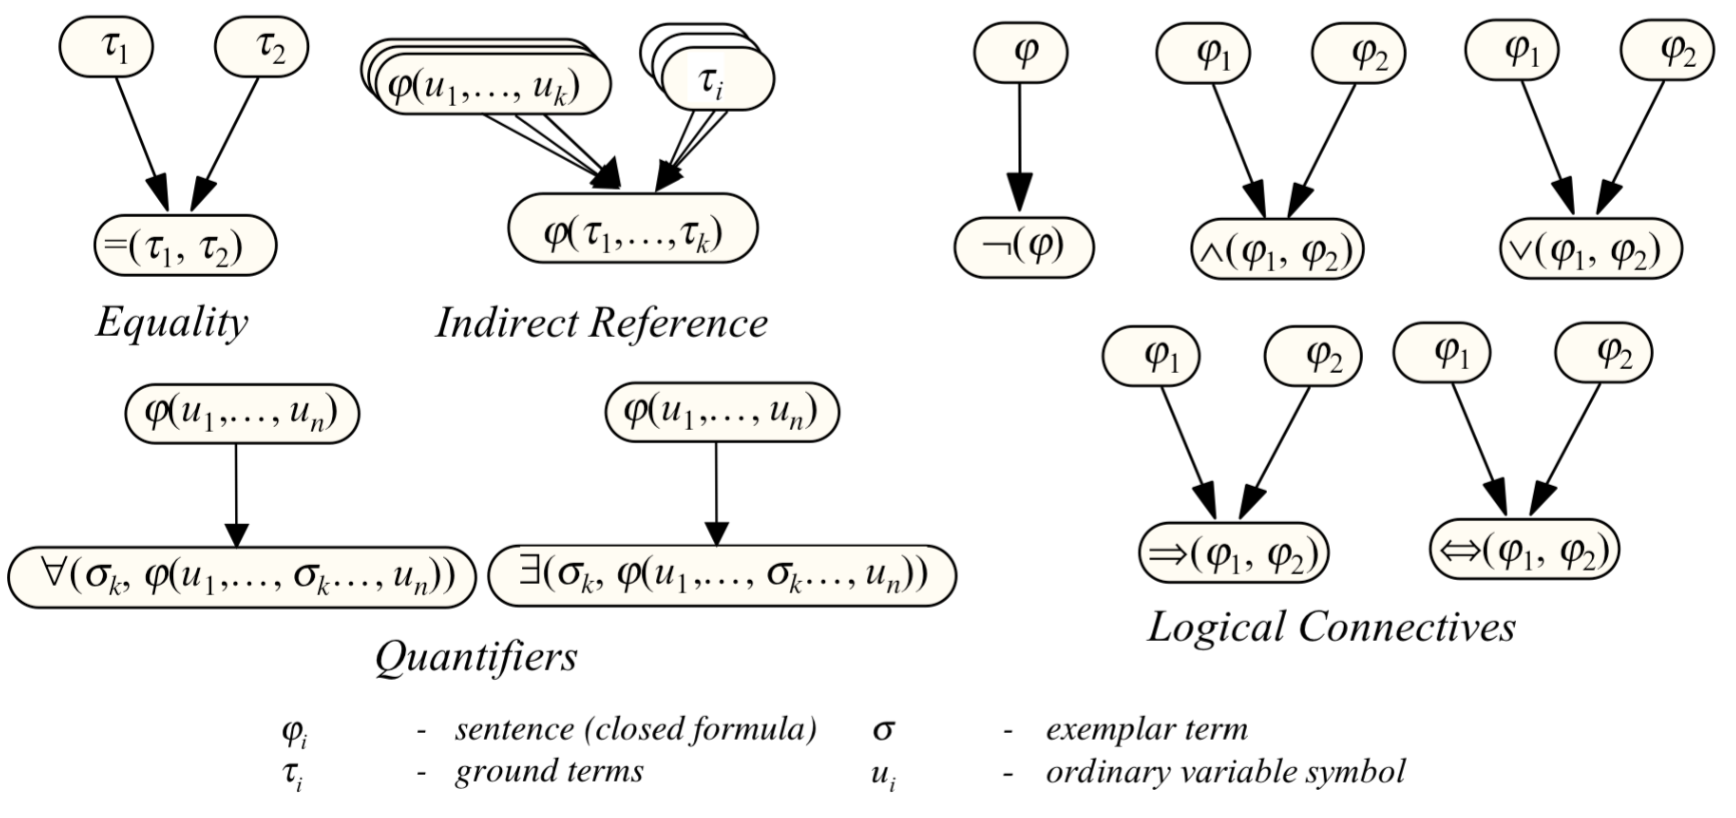
\includegraphics[height=5cm]{./images/sentences}
	\caption{Logical MFrags}
	\label{fig:sentences}
\end{figure}

Um MFrag pode ser definido com 5 componentes:
\begin{itemize}
	\item $C$: Conjunto finito de valores de contexto
	\item $I$: Conjunto finito de termos de variáveis de entrada
	\item $R$: Conjunto finito de termos de variáveis residentes
	\item $G$: Um grafo direcionado acíclico
	\item $D$: Distribuições de probabilidades locais para cada variável no conjunto $R$
\end{itemize}

Por exemplo, na figura~\ref{fig:mfrag}, os valores de contexto estão em cor amarelo, em cinza as variáveis de entrada e em branco as variáveis residentes. As tabelas em cada nó do grafo representam suas distribuições de probabilidades locais.

\begin{figure}
	\centering
	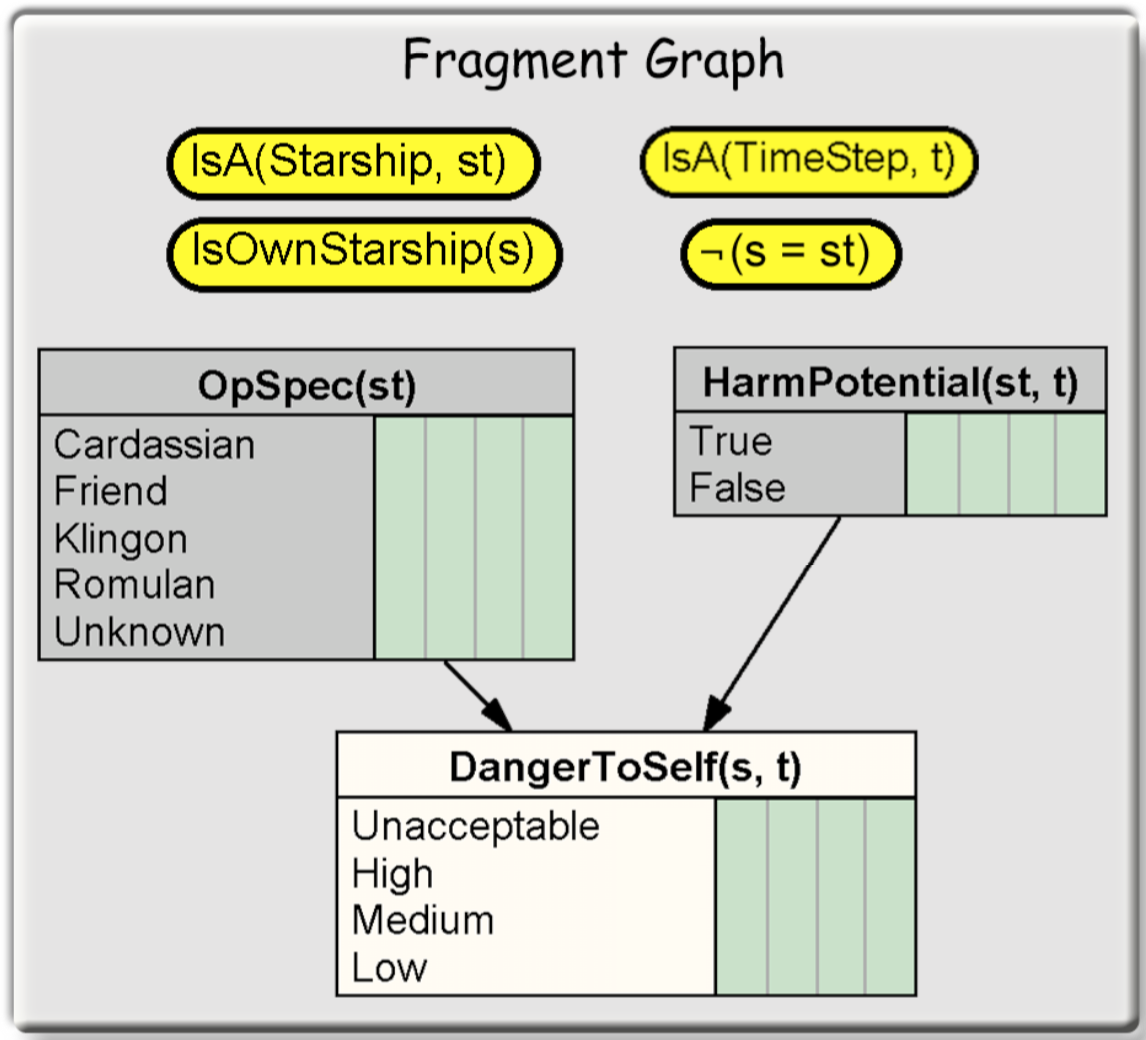
\includegraphics[height=5cm]{./images/mfrag}
	\caption{DangerToSelf MFrag}
	\label{fig:mfrag}
\end{figure}